\begin{exercise}{trigonometrie.sinus}{Sinus}
  \ifproblem\problem\par
    Bestimme die angegebenen Werte der Sinus-Funktion ohne Taschenrechner.
    \begin{center}
      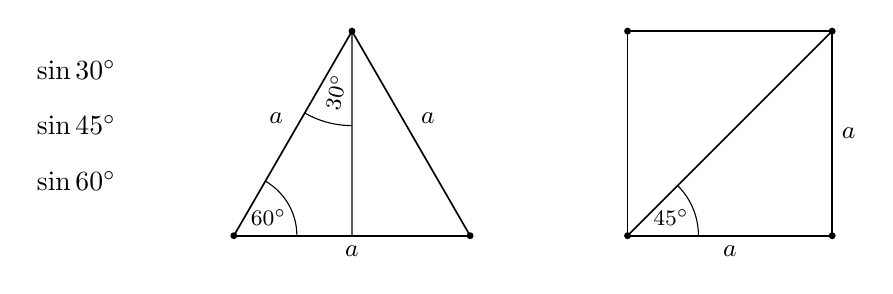
\begin{tikzpicture}
        \begin{scope}
          \node at (0, 2.1) {{$\sin 30^{\circ}$}};
          \node at (0, 1.4) {{$\sin 45^{\circ}$}};
          \node at (0, 0.7) {{$\sin 60^{\circ}$}};
        \end{scope}
        \begin{scope}[xshift=2cm]
          \coordinate (A) at (0.0, 0.0);
          \coordinate (B) at (3.0, 0.0);
          \coordinate (C) at (60:3.0cm);
          \coordinate (S) at (1.5, 0.0);
          % Dreiecksseiten
          \draw[line width=0.6pt] (A) -- node[below]{{\small$a$}}       (B);
          \draw[line width=0.6pt] (B) -- node[above right]{{\small$a$}} (C);
          \draw[line width=0.6pt] (C) -- node[above left]{{\small$a$}}  (A);
          % Hoehe
          \draw (C) -- (S);
          % Eckpunkte
          \fill (A) circle[radius=1.25pt];
          \fill (B) circle[radius=1.25pt];
          \fill (C) circle[radius=1.25pt];
          % Winkel
          \begin{scope}
            \clip (A) -- (S) -- (C) -- cycle;
            \draw[line width=0.4pt] (A) circle[radius=8mm];
            \draw[line width=0.4pt] (C) circle[radius=12mm];
            \node[shift=(255:8mm), rotate=77] at (C) {{\footnotesize$30^{\circ}$}};
            \node[shift=(28:5mm)] at (A) {{\footnotesize$60^{\circ}$}};
          \end{scope}
        \end{scope}
        \begin{scope}[xshift=7cm]
          \coordinate (A) at (0.000, 0.000);
          \coordinate (B) at (2.598, 0.000);
          \coordinate (C) at (2.598, 2.598);
          \coordinate (D) at (0.000, 2.598);
          % Quadrat
          \draw[line width=0.6pt] (A) -- (B) -- (C) -- (D) -- (A);
          % Bezeichnungen
          \path (A) -- node[below]{{\small$a$}} (B);
          \path (B) -- node[right]{{\small$a$}} (C);
          % Diagonale
          \draw[line width=0.6pt] (A) -- (C);
          % Eckpunkte
          \fill (A) circle[radius=1.25pt];
          \fill (B) circle[radius=1.25pt];
          \fill (C) circle[radius=1.25pt];
          \fill (D) circle[radius=1.25pt];
          % Winkel
          \begin{scope}
            \clip (A) -- (B) -- (C) -- cycle;
            \draw[line width=0.4pt] (A) circle[radius=9mm];
            \node[shift=(22.5:6mm)] at (A) {{\footnotesize$45^{\circ}$}};
          \end{scope}
        \end{scope}
      \end{tikzpicture}
    \end{center}
  \fi
  %\ifoutline\outline\par
  %\fi
  %\ifoutcome\outcome\par
  %\fi
\end{exercise}
